\documentclass[9pt,twocolumn,twoside,lineno]{pnas-new}
% Use the lineno option to display guide line numbers if required.

\templatetype{pnasresearcharticle} % Choose template 
% {pnasresearcharticle} = Template for a two-column research article
% {pnasmathematics} %= Template for a one-column mathematics article
% {pnasinvited} %= Template for a PNAS invited submission

% Math
\def\P{\mathbb{P}}
\def\cor{\mathrm{cor}}
\def\Quantile{\mathrm{Quantile}}
\def\logit{\mathrm{logit}}
\def\dist{\mathrm{dist}}
\def\WIS{\mathrm{WIS}}
\def\AUC{\mathrm{AUC}}
\newcommand{\indicator}[1]{\mathbf{1}\left(#1\right)}

% Figures and tables
\usepackage{xurl}
\usepackage{microtype}
\usepackage{booktabs}
\usepackage{caption}
\usepackage{subcaption}
\usepackage{xcolor}
\newcommand{\attn}[1]{\textcolor{red}{[ATTN: #1]}}

\makeatletter 
\renewcommand\@biblabel[1]{#1} 
\makeatother

% indicators
\newcommand{\chngcli}{CHNG-CLI}
\newcommand{\chngcov}{CHNG-COVID}
\newcommand{\dv}{DV-CLI}
\newcommand{\ar}{AR}
\newcommand{\fb}{CTIS-CLI-in-community}
\newcommand{\gs}{Google-AA}


\title{Can Auxiliary Indicators Improve COVID-19 Forecasts and Hotspot
  Prediction?} 

% Use letters for affiliations, numbers to show equal authorship (if applicable) and to indicate the corresponding author
\author[a,c,1]{Author One}
\author[b,1,2]{Author Two} 
\author[a]{Author Three}

\affil[a]{Affiliation One}
\affil[b]{Affiliation Two}
\affil[c]{Affiliation Three}

% Please give the surname of the lead author for the running footer
\leadauthor{Lead author last name} 

% Please add a significance statement to explain the relevance of your work
% TODO write one. This is the indicator's one.
\significancestatement{To study the COVID-19 pandemic, its effects on society,
  and measures for reducing its spread, researchers need detailed data on the
  course of the pandemic. Standard public health data streams suffer
  inconsistent reporting and frequent, unexpected revisions. They also miss
  other aspects of a population's behavior, worthy of consideration. We
  present an open database of COVID signals in the United States, measured at
  the county level and updated daily. These include traditionally reported COVID
  cases and deaths, and many others: signals based on measures of mobility,
  social distancing, internet search trends, self-reported symptoms, and
  patterns COVID-related activity in de-identified medical insurance claims. The
  database provides all signals in a common, easy-to-use format, empowering both
  public health research and operational decision-making.
}

% Please include corresponding author, author contribution and author
% declaration information 
\authorcontributions{Please provide details of author contributions here.}
\authordeclaration{Please declare any competing interests here.}
\equalauthors{\textsuperscript{1}A.O.(Author One) contributed equally to this
  work with A.T. (Author Two) (remove if not applicable).} 
\correspondingauthor{\textsuperscript{2}To whom correspondence should be
  addressed. E-mail: author.two\@email.com} 

% At least three keywords are required at submission. Please provide three to
% five keywords, separated by the pipe symbol. 
\keywords{Keyword 1 $|$ Keyword 2 $|$ Keyword 3 $|$ ...} 

\begin{abstract}
Please provide an abstract of no more than 250 words in a single paragraph.
Abstracts should explain to the general reader the major contributions of the
article. References in the abstract must be cited in full within the abstract
itself and cited in the text. 
\end{abstract}

\dates{This manuscript was compiled on \today}
\doi{\url{www.pnas.org/cgi/doi/10.1073/pnas.XXXXXXXXXX}}

\begin{document}

\maketitle
\thispagestyle{firststyle}
\ifthenelse{\boolean{shortarticle}}{\ifthenelse{\boolean{singlecolumn}}{\abscontentformatted}{\abscontent}}{}

\dropcap{T}racking and forecasting indicators from public health reporting
streams---such as confirmed cases and deaths in the COVID-19 pandemic---is
crucial for understanding disease spread, formulating public policy responses,
and anticipating future public health resource needs.  In a companion paper, we
describe our research group's (Delphi's) efforts in curating and maintaining a 
database of real-time indicators that track COVID-19 activity and other relevant
phenomena. The signals (a term we use synonomously with ``indicators'') in this
database are accessible through the COVIDcast API \cite{CovidcastAPI}, with
associated R \cite{CovidcastR} and Python \cite{CovidcastPy} packages for
convenient data fetching and processing tools. In the current paper, we aim to
quantify the utility provided by a core set of these indicators for two
fundamental prediction tasks: probabilistic forecasting of COVID-19 case 
rates and prediction of future COVID-19 case hotspots (defined by the event that
a relative increase in COVID-19 cases exceeds a certain threshold). 

At the outset, we should be clear that our intent in this paper is \textit{not}
to provide an authoritative take on cutting-edge COVID-19 forecasting methods.
Instead, our purpose here is to provide a rigorous, quantitative assessment of
the utility that several auxiliary indicators---such as those derived from
internet surveys or medical insurance claims---provide in tasks that involve
predicting future trends in confirmed COVID-19 cases. To assess such utility in
as simple terms as possible, we center our study in the framework of a basic
autoregressive model (in which COVID cases in the near future are predicted from  
a linear combination of COVID cases in the near past), and ask whether the 
inclusion of an auxiliary indicator as an exogenous feature in such a model
improves predictive power. While forecasting carries a rich literature that
offers a wide range of techniques, see e.g., \cite{Hyndman:2018}, we purposely
constrain ourselves to very simple models, avoiding common enhancements such as
order selection, correction of outliers/anomalies in the data, and inclusion of
regularization or nonlinearities. That said, analyses of forecasts submitted to
the COVID-19 Forecast Hub \cite{ForecastHub} by a large community of modelers
have shown that simple, robust models have consistently been among the
best-performing over the pandemic \cite{Cramer:2021}, including time series
models similar to those we consider in what follows.  

In our companion paper, we analyze correlations between various indicators and   
COVID case rates. These correlations are natural summaries of the
contemporaneous association between an indicator and COVID cases, but they fall 
short of delivering a satisfactory answer to the question that motivates the
current article: is the information contained in an indicator demonstrably
useful for the prediction tasks we care about? For such a question, lagged
correlations (e.g., measuring the correlation between an indicator and COVID
case rates several days in the future) move us in the right direction, but still
do not move us all the way there. The question about \textit{utility for 
  prediction} is focused on a much higher standard than simply asking 
about correlations; to be useful in forecast or hotspot models, an indicator
must provide relevant information that is not otherwise contained in past values
of the case rate series itself. We will assess this in the most direct way
possible: by inpsecting the difference in predictive performance of simple
autoregressive models trained with and without access to past values of a
particular indicator.   

There is another, more subtle issue in evaluating predictive utility that 
deserves explicit mention, as it will play a key role in our analysis.
Signals computed from surveillance streams will often be subject to  
latency and/or revision. For example, a signal based on aggregated medical
insurance claims may be available after just a few days, but it can then be
substantially revised over the next several weeks as additional claims are
submitted and/or processed late. Correlations between such a signal and case
rates calculated ``after the fact'' (computed retrospectively, using the
finalized values of this signal) will not deliver an honest answer to the    
question of whether this signal would have been useful in real time. Instead,
we build predictive models using only the data that would have been available
\textit{as of} the prediction date, and compare the ensuing predictions in terms 
of accuracy. To do so, we leverage Delphi's \texttt{evalcast} R package 
\cite{EvalcastR}, which plugs into the COVIDcast API's data versioning system,  
and facilitates honest backtesting. 

% Furthermore, adopting this practically-oriented forecasting
% perspective to indicator evaluation requires one to confront
% fundamental limitations inherent to public health surveillance
% systems.  In particular, many reporting systems are plagued by
% latency, with delays in reporting that can sometimes span
% multiple weeks.  Latency manifests itself in different ways in different data sources.  Some data sources may only make a signal available one week after the date it describes; other
% data sources may provide immediate imperfect initial estimates, which are
% gradually ``backfilled'' over a period of days, weeks, or months (in which previous estimates are updated as new
% data trickle in).  And few of
% these latency patterns are stable or predictable, with holidays,
% extreme weather events, and changes in the reporting process all
% affecting the dynamics of the delay process.  To fully and accurately
% understand an indicator's usefulness for forecasting requires
% accounting for the unfortunate reality of data latency.

% Examining the importance of additional features for prediction is a core question
% in inferential statistics, and there are many ways to examine this question
% under a variety of assumptions. For time series, work in
% this area can be traced at least to Granger causality~\cite{GrangerCausality} and
% related multivariate extensions~\cite{GewekeTimeSeries} under the condition 
% that the series are linearly related autoregressions among other assumptions.
% These techniques are especially popular in econometrics and neuroscience~\cite{mccracken2007asymptotics,NeuroscienceGranger}.

% We choose to take a
% predictive angle, which is simple but also fairly robust, compared to various
% other classical inferential approaches. In fact, drawing rigorous inference based on
% predictions, without (or with lean) assumptions, is an active field of
% research~\cite{dai2021significance,fryer2021shapley,zhang2020floodgate,williamson2020unified}.
% Nonetheless, the predictive approach directly examines the target of interest: do
% these signals help to produce forecasts? Furthermore, directly comparing
% forecast errors without strong assumptions through tests of predictive accuracy
% are common in epidemiology, econometrics, and other
% fields~\cite{DieboldMarianoTest,DieboldRetrospective}. 

% - then make the broad point that "feature importance" is a core question in
% statistics, and there are many ways to look at it and lots of literature (cite
% a bunch fo stuff).  We choose to take a predictive angle, which is simple but
% also fairly robust, compared to various other classical inferential approaches
% that make lots of assumptions.  In fact, drawing rigorous inference based on
% predictions, without (or with lean) assumptions, is an active field of
% research.  Cite several papers (Jing's conformal paper that describes LOCO,  
% commentary by Ale, Ryan, Larry in Stat Sci, a bunch of model X stuff including
% Lukas Janson's recent paper, Eugene + Aaditya's recent paper?).  Larry has put
% some references in the bib.  Put more if we can find them, especially on time
% series. 

\section{Methods}

\subsection{Signals and Locations}

We consider prediction of future COVID-19 case rates or case hotspots (to be
defined precisely shortly).  By case rate, we mean the case count per 100,000
people (the standard in epidemiology).  We use reported case data aggregated by 
JHU CSSE \cite{Dong:2020}, which is accessible through the COVIDcast API, like
the auxiliary indicators that we use to supplement the basic purely
autoregressive models.   

The indicators we focus on provide information not generally available from
standard public health reporting. Among the many indicators in the API, we
consider the following five:
\begin{itemize}
\item Change Healthcare COVID-like illness (CHNG-CLI): The percentage of
  outpatient visits that are primarily about COVID-related symptoms, based on
  de-identified Change Healthcare claims data.
\item Change Healthcare COVID (CHNG-COVID): The percentage of outpatient visits
  with confirmed COVID-19, based on the same claims data.
\item COVID Tracking and Impact Survey CLI-in-community (CTIS-CLI-in-community): 
  The estimated percentage of the population who knows someone who is sick,
  based on Delphi's surveys of Facebook users.
\item Doctor Visits COVID-like illness (DV-CLI): The same as CHNG-CLI, but
  computed based on de-identified medical insurance claims from other health
  systems partners.  
\item Google Search Trends for anosmia and ageusia (Google-AA): A measure of 
  COVID-19 related Google search volume for queries related to anosmia (loss of
  smell), ageusia (loss of taste), or both.  
\end{itemize}
In short, we choose these indicators because, conceptually speaking, they
measure aspects of an individual's disease progression that would plausibly
precede the occurence of (at worst, co-occur  with) the report of a positive
COVID-19 test, through standard public health reporting streams.

For more details on the five indicators (including how these are precisely
computed from the underlying data streams) we refer to
\url{https://cmu-delphi.github.io/delphi-epidata/api/covidcast_signals.html},
which documents all of the COVIDcast signals, as well our companion paper on 
COVIDcast API and database. For CTIS in particular, we refer to our companion 
paper on this survey. For the Google Search Trends data set, see
\cite{GoogleSymptoms}, and \cite{Klopfen:2020, Vaira:2020} for articles on the
relevance of anosmia and ageusia.  

As for geographic resolution, we consider the prediction of COVID-19 case rates
and hotspots aggregated at the level of an individual \textit{hospital referral
  region} (HRR). HRRs correspond to groups of counties in the United States
within the same hospital referral system. The Dartmouth Atlas of Healthcare 
Policy~\cite{DartmouthHRR}, defines these 306 regions based on a number of
characteristics. They are contiguous regions containing at least one city where
major procedures (cardiovascular or neurological) are performed.  Most hospital
services for the population in an HRR are performed by hospitals within the
region.  Each HRR has a minimum population of about 120,000; some HRRs are quite
large (such as the one containing Los Angeles, which has about 10 million
people), but generally HRRs are much more homogenous in size than the
(approximately) 3200 counties are, and they serve as a nice middle ground in 
between counties and states. 

HRRs, by their definition, would be most relevant for forecasting hospital
admissions.  We have chosen to focus on cases (forecasting and predicting
hotspots) at this resolution since the indicators considered should be more
useful in predicting case versus hospitalization activity, the latter being
intuitively more closely connected (in time) to the events that are measured by
the given five indicators. Predicting case rates (and hotspots) at the HRR level
is still a reasonable goal in its own right; and moreover, it could be used to
feed predicted case information into downstream hospitalization models.

\subsection{Vintage Training Data}

In this paper, all models are fit using only ``vintage'' training data. This
means that for a given prediction date, say September 1, 2020, we train models
using only the data that would have been available to us \textit{as of}
September 1.  Essentially, we ``rewind'' the clock to September 1, and query the
COVIDcast API to get the latest data that it would have had available at
that point in time.  This is made possible by the COVIDcast API's comprehensive
data versioning system (described in more detail in our companion paper).  We
also use the \texttt{evalcast} R package \cite{EvalcastR}, which streamlines the
process of training arbitrary prediction models over a sequence of prediction
dates, by automatically constructing the (properly-versioned) sequence of
vintage training data sets.  

Vintage training data means different things, in practice, for different
signals. The three signals based on medical claims, CHNG-CLI, CHNG-COVID, and
DV-CLI, are most often 3-5 days latent, and subject to a considerable degree of
revision or ``backfill'' after their initial publication date.  The survey-based
signal, CTIS-CLI-in-community, is 2 days latent, and rarely undergoes any 
revision at all.  The target itself, reported case rates (or a binary hotspot
variable, defined based on reported case rates), is 1 day latent, and exhibits
frequent, unpredictable revisions (sometimes clear anomalies) after initial
publication.  Compared to the revision pattern in the medical claims signals,
which are appears to be much more systematic, the revision pattern in the case
rates signal can be highly erratic, resulting in big spikes as reporting
backlogs are cleared, changes in case definitions are made, other corrections
are applied, etc.

TODO What is ground truth??
TODO Better example of backfill in DV-CLI?

\subsection{Analysis Tasks}

%\subsubsection{Forecasting Commonalities} % PNAS wants Title Caps for everything 

On every day between \attn{July 1 and December 31}, we make two types of
forecasts for each of the 306 hospital referral regions in the United States:
(1) we forecast the seven-day trailing average of incident cases, or "smoothed
incident cases"; and (2) we predict whether the HRR will be a hotspot, a
location with a large increase in cases. For both tasks we try to predict the
outcome 7, 8, 9, up to \attn{21} days into the future. For both tasks, we
estimate a baseline global model across all HRRs using the most recent
observation of the target, as well the observations from 1 and 2 weeks earlier.
We train a separate model for each forecast date and for each forecast horizon,
but we do not assume any HRR-specific effects; that is, a single global model is
used to 
describe all HRRs for each forecast date-horizon pair. This model is
re-estimated for every forecast date and each future target resulting in
\attn{$180\times 15 = 2700$} estimated baseline models for each task.  
We then add current and lagged values (analogous to the baseline) for each of
the four signals separately. We now provide further details on each of these
tasks. 

\subsubsection{Task 1: Case Forecasting}

To fix notation, let $Y_{\ell,t}$ denote the smoothed COVID-19 case
incidence rate per 100,000 people for location (HRR) $\ell$ and time (day) $t$. 
Let $X_{\ell,t}$ denote
the one of the indicators described above, for example the Facebook \%
CLI-in-community signal, 
for location $\ell$ and time $t$.
We evaluate five models of the form:
\begin{align*}
Y_{\ell,t+d}
&\approx \alpha + \sum_{j=0}^2 \beta_j Y_{\ell,t-7j} \\
Y_{\ell,t+d}
&\approx \alpha + \sum_{j=0}^2 \beta_j Y_{\ell,t-7j} +
\sum_{j=0}^2 \gamma_j X_{\ell,t-7j}, 
\end{align*}
where we also exchange $X_{\ell, t}$ for the signals from \attn{CHNG and
  Google.} 
Here $d=7,\ldots, 21$ depending on the target value
(number of days ahead we predict).

Informally, the first model, which we will call the ``Cases'' model, 
bases its predictions of future case rates on the following three features:
current COVID-19 case rates and those 1 and 2 weeks back.
The second model, ``Cases + Facebook'', additionally incorporates the 
current Facebook signal and the Facebook signal from 1 and 2 weeks in the past.
The third model, ``Cases + Google'', is exactly the same but substitutes the 
Google signal instead of the Facebook one and similarly for ``Cases + Change''.


For each model, in order to make a forecast at time $t_0$
(to predict case rates at time $t_0+d$),
we estimate the unknown parameters using quantile
regression~\cite{KoenkerXiao2006}, 
training over all locations $\ell$,
and all times $t$ that are within the most recent 21 days of data
available up to and including time $t_0$.
Rather than predicting only the median (or mean) value for each forecast date
and each horizon, we estimate seven quantiles, coinciding 
with the county-level forecast submission guidelines for the
COVID-19 Forecast Hub~\cite{Cramer:2021}.  These are \{0.025, 0.1,
0.25, 0.5, 
0.75, 0.9, 0.975\}. This provides a notion of uncertainty in the forecasts. An
example of this type of forecast is shown in \autoref{fig:trajectory}. 

\begin{figure}[tb!]
    \centering
    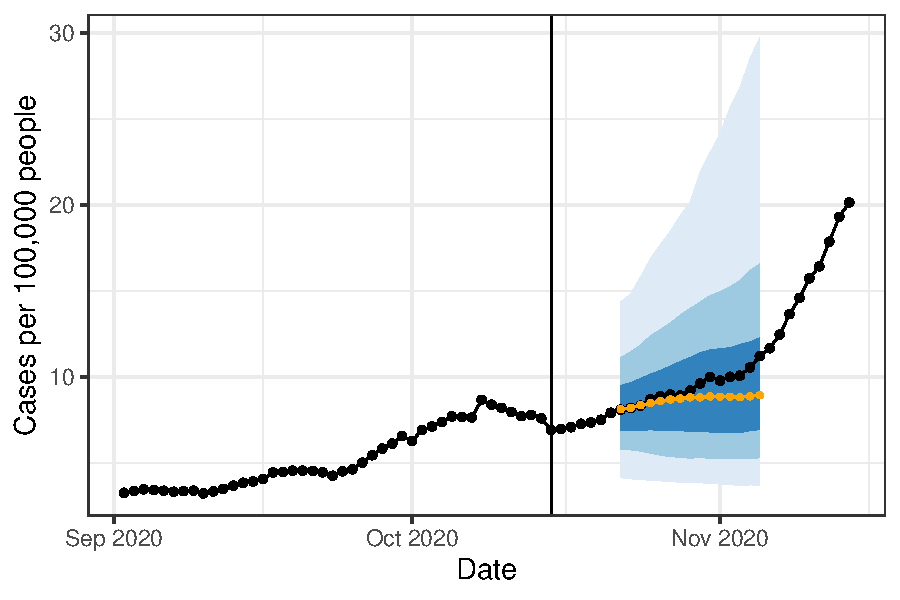
\includegraphics[width=.9\linewidth]{fig/trajectory.pdf}
    \caption{Forecasts and observed cases for HRR x. \attn{Create a figure here
        for 1 HRR. Show the fan for the quantiles.}} 
    \label{fig:trajectory}
\end{figure}




% Noncrossing is enforced via post hoc ordering.

\subsubsection{Task 2: Hotspot Prediction}

We also examine whether alternative indicators help in predicting hotspots. On a
given date, we say an HRR is a hotspot if the average number of observed cases
over the past 7 days has increased by at least $25$\% compared to the preceding
week. We remove all data where, on average, fewer than $30$ cases were observed
over the preceding $7$ days. Thus, hotspot status can be represented by a
$\{0,1\}$-valued variable, and hotspot prediction is a binary classification
problem.  

As in the case forecasting task, in hotspot prediction we train models that use
previously observed values of cases and alternative indicators as features to
predict a response (in our case, hotspot status). In addition to the differently
defined response, there are two other differences between the hotspot prediction
and case forecasting tasks. First, in hotspot prediction we always use relative
changes in previous observed cases/indicators as features. That is, rather than
$Y_{t,\ell}$ we use 
$$
Y^\Delta_{\ell,t} = \frac{Y_{\ell,t} - Y_{\ell,
    t-7}}{Y_{\ell,t-7}}\quad\text{and}\quad X^\Delta_{\ell,t} =
\frac{X_{\ell,t} - X_{\ell, t-7}}{X_{\ell,t-7}} 
$$ 
Second, because hotspot prediction is a binary classification problem, we
estimate the parameters $\alpha$, $\beta$ and $\gamma$ by logistic regression
rather than quantile regression. 

\subsection{Evaluation Metrics}

We evaluate forecasts for each forecast date and horizon using the weighted
interval score. Weighted interval score (WIS), a well-known quantile-based
approximation of the commonly-used continuous ranked probability
score~\cite{gneiting-proper-score}. WIS is a proper score, meaning that lower
scores imply better forecasters, and can be thought of as a distributional
generalization of absolute error. The CDC has embraced this metric in the
context of epidemic forecasting and especially for COVID-19~\cite{wis-paper}.
Essentially, pairs of quantile forecasts are treated as a central  interval. For
example, the 0.1 and 0.9 quantiles create an 80\% interval that should, if the
forecaster is well-calibrated, contain the truth about 80\% of the time. A
forecaster whose 80\% interval contains the truth less frequently is overly
confident, while one whose interval contains the truth more frequently (say, by
using an infinitely-wide interval) is failing to take a stand on the future
outcome.  

Here, denoting $K$ predicted intervals along with the median  as
$\{\alpha_K/2,\ldots,\alpha_2/2,\  
\alpha_1/2,\ 0.5, 1-\alpha_1/2,\ 1-\alpha_2/2,\ldots, 1-\alpha_K/2\}$, the associated
forecasts as $\{l_K,\ldots, l_2,\ l_1,\ m,\ u_1,\ u_2,\ldots, u_K \}$, and the observed
value (after the forecast was made) as $y$, this metric can be expressed as
\attn{someone please check this} 
\begin{align*}
 \operatorname{WIS}_K &= \frac{1}{K}|m -y | + \frac{2}{K+1}\sum_{k=1}^K 
\frac{1}{\alpha_k}(u_k - l_k)\\ &\quad + \sum_{k=1}^K  
(l_k - y)\indicator{y < l_k} +
(y - u_k)\indicator{y> u_k},
\end{align*}
where $\indicator{a} = 1$ if $a$ is true and $0$ otherwise. Essentially, this
metric decomposes into 4 parts: (1) a penalty for the median, the point forecast
or best guess, being far from the truth; (2) a penalty for the width of each
interval ($u_k - l_k$); (3)  a penalty for overprediction, when the observed
value falls below $l_k$ and hence underneath the interval; and (4) a
corresponding penalty for underprediction. Weighted interval score can also be
written in terms of an average of the quantile or ``pinball'' losses. Setting $\tau_1 =
\alpha_K/2,\ \ldots,\ \tau_{K+1} = 0.5,\ \ldots,\ \tau_{2K+1} = 1-\alpha_K/2$ and
similarly rewriting $q_1 = l_K,\ \ldots,\ q_{K+1}=m,\ \ldots,\ q_{2K+1}=u_K$, then
\begin{align*}
  \operatorname{WIS}_K &= \frac{2}{2K+1} \sum_{k=1}^{2K+1}
                         \left(\indicator{y \leq q_k} -\tau_k\right)
                         (q_k - y).
\end{align*}
While this second expression does not have the convenient decomposition
discussed above, the pinball loss is precisely the objective function that
quantile regression minimizes. So, mathematically, quantile regression should
give parameter estimates that minimize the in-sample weighted interval score.
% DJM: In trying to figure out where 'pinball' comes from, it looks like the
% preprint of the massively cited Koenker and Hallock (2001) JEP article. See
% http://www.econ.uiuc.edu/~roger/research/intro/rq.pdf. They say that tilting
% the absolute value is `pinball logic' which is not a connection I would have
% ever made. The language doesn't seem to have made it to the final version.
% Maybe there's an earlier reference?


When comparing the aggregate performance of the baseline quantile autoregression
without additional signals with 
the indicator-assisted quantile autoregression forecasters, we first
normalize the individual weighted interval scores by the weighted interval
score of a boneheaded model: predicting all future values to be the same as the
most recent observation. The dummy model uses the errors such a forecast has
made in-sample to form the other quantiles. We normalize by 
the dummy model to account for the fact that different locations or
time periods have different magnitudes of COVID-19 incidence (even after
scaling by population). Performing well by this metric means that a particular
forecaster is doing well at all locations and time periods. Without the scaling,
a forecaster that is good at locations and time periods with relatively high
case numbers but poor everywhere else could appear preferable. 

For hotspots, we use the area under the curve (AUC) computed by examining the
true-positive and false-negative rates across HRRs at each horizon and forecast
date. That is, for a particular forecast date and a particular horizon, we ask,
how many true hotspots were called hotspots compared to the total number of
hotspots (specificity). The false-negative rate (sensitivity) is the ratio of
correctly classified non-hotspots to the total number of non-hotspots. A perfect
classifier would have both sensitivity and specificity equal to 1. Plotting the
sensitivity on the $y$-axis and $1-$specificity on the $x$-axis where each point
is a forecast date produces an ROC curve for each classifier. We compute the
area under this curve for each forecast horizon to compare the cases-only model
to those adding indicators. 




\paragraph{\attn{Methods section graveyard, most for Appendix}}

\begin{itemize}
\item Discuss the "how many days does the indicator buy" interpretation here or below? 


\item Do we explain why regularization/CV not really helpful for both
forecasting and hotspots


\item Implementation was via quantgen, cite here?

\item some people don't like relative WIS beacuse it's no longer a
``proper score''.  directly address that here?


\item Do we talk about log loss?

\item Do we explain that we are using infinite-backfilled data?


\end{itemize}



\section{Results}

Code to reproduce all examples (which uses the
\texttt{evalcast} R package and fetches data directly from the API) can be
found at \url{TODO}.

\subsection{Primary Results}

Figure \ref{fig:topline-overall-results} displays the primary results
of this paper, showing the effect of using indicators on the two
forecasting tasks as a function of the horizon of the forecast (i.e.,
the number of days ahead one is forecasting). For the case rate forecasting
task, the left panel shows the ratio of the mean
WIS 
of each forecaster relative to the mean WIS of the
baseline. \attn{Further description and justification of this metric
  should be added to the ``Evaluation Metrics'' section rather than
  here it seems?}  Both means are taken over all HRRs and forecast
dates ranging from June 9, 2020 to December 31, 2020 \attn{verify}.
All curves are well below 1, which means that all methods, including \ar, outperform the baseline across all
considered forecast horizons. The claims-based
indicators \dv~and \chngcov~show the most substantial gains, whereas
the \chngcli~does not show any improvement over \ar.  The \fb~and
\gs~indicators also show a non-negligible improvement.  Notably,
\fb~is the only indicator to offer a clear improvement at far aheads.
%\begin{itemize}
%\item \dv~and \chngcov~perform very well
%\item \fb~and \gs~perform well
%\item \chngcli~performs poorly
%\item Interestingly, fb is the only one offering clear improvement at
 % far aheads
%\item Note the y-axis: consistent, clear improvement over baseline
%\end{itemize}

For the hotspot prediction task, the right panel of Figure
\ref{fig:topline-overall-results} shows the AUC of each method.
The monotonic decrease of all curves reflects the fact that hotspot
prediction gets harder as the forecasting horizon increases. At the
highest considered ahead (nearly one month ahead), the AUCs are close
  to 0.5, which is no better than random guessing.
In the 7-14 day ahead range, the indicators show a noticeable
  improvement over \ar.  For larger horizons there does not
  appear to be much difference in methods.
The approximate ordering of methods is similar to what is seen
  in the forecasting task: \chngcov~and \dv~are the strongest
  performing and \ar~the weakest.
Even for 7-day ahead predictions, the AUC is below 0.7,
  suggesting that all methods struggle with this classification
  task. \attn{Do people agree that an AUC of 0.7 is not all that great?}
  That said, \dv~and \chngcov~attain roughly a 10\% increase in AUC
  over the \ar~classifier.
  
%\begin{itemize}
%\item Monotonic decrease reflects the fact that hotspot
%  prediction gets harder as ahead increases.
%\item At the highest ahead (almost one month ahead) the AUCs are close
%  to 0.5, which is no better than random guessing.
%\item In the 7-14 day ahead range, the indicators show a noticeable
%  improvement over the \ar.  For larger horizons there does not
%  appear to be much difference in methods
%\item The approximate ordering of methods is similar to what is seen
%  in the forecasting task: chng\_cov and dv are the strongest
%  performing and \ar the weakest.
%\item Even for 7-day ahead predictions, the AUC is below 0.7,
%  suggesting that all methods struggle with this classification task.
%  That said, dv and chng\_cov attain roughly a 10\% increase in AUC
%  over the \ar classifier.
%\end{itemize}


% We see that all three \attn{will need to
% include imputed-zero google here, hopefully four} indicator-assisted
% forecasters improve upon the baseline QAR3 forecaster.  The QAR3 model
% assisted by the Change Healthcare confirmed COVID-19 signal
% (QAR3+CHCOV3) sees the strongest improvement.
% C`

\begin{figure}[tb!]
  \centering
  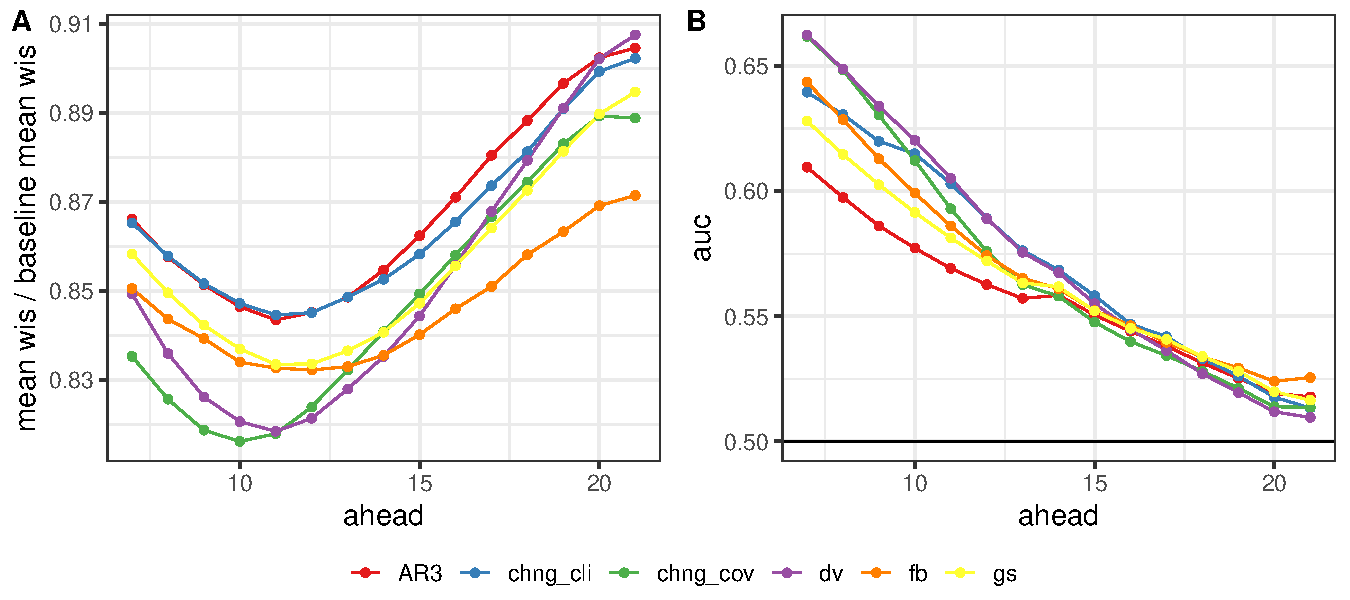
\includegraphics[width=\linewidth]{fig/figure5.pdf}
  \caption{\label{fig:topline-overall-results}  Forecasting performance as a
    function of number of days 
    ahead, aggregated across all HRRs and forecast dates. \attn{How's this?}}
\end{figure}

\subsection{Avoiding misleading retrospective evaluations}

Figure \ref{fig:finalized-vs-honest} quantifies the effect of
not properly accounting for the question of ``what was known when'' in
performing retrospective evaluations of forecasters.  When methods are
given the finalized version of the data rather than the version available at the time that the forecast would have been made, all methods
appear (falsely) to have better performance.  For example, for forecasting case rates
7-days ahead, the WIS of all methods is at least 8\% larger than what would have been
recorded using the finalized values of the data.  This effect
diminishes as the forecasting horizon increases, reflecting the fact
that these forecasters rely less heavily on recent data than very
short-term forecasters.  Crucially, some methods are
``helped'' more than others by the less scrupulous retrospective
evaluation, underscoring the difficulty of avoiding misleading
conclusions when performing retrospective evaluations of forecasters.

The \chngcli~indicator (along with the other claims-based signals) is the most
affected by this distinction, reflecting the latency in claims-based
reporting. \attn{Actually, \dv~is the least affected for forecasting
  whereas it is one of the most affected for hotspots.}  This supports
the importance of efforts to provide ``nowcasts'' for claims signals
(which corresponds to a 0-ahead ``forecast'' of what the claims
signal's value will be once all data has been collected).

Even the \ar~model is affected by this distinction, reflecting the
fact that the case rates themselves (i.e., the response values) are also
subject to revision.  The forecasters based on indicators are thus
affected both by revisions to the indicators and by revisions to the
case rates.

\begin{itemize}
%\item Motivates the importance of nowcasting for claims signals.
  \item For forecasting task: Also, \chngcli~and \dv~perform very similarly here, which is
    reassuring because they're measuring the same thing (in
    principle).  Yet they must have very different backfill profiles…
  \item For hotspots task: dv seems to get a bigger boost than
    \chngcov - interesting dichotomy to forecasting
\item But in both forecasting/hotspots \chngcli~is affected a lot by backfill
\item \attn{We should be careful about which indicators we were not
      able to track latency for.  In fact, we should probably remove
      these from the plot since they would be more strongly affected
      than is shown in the plot.}

\item \attn{We can also discuss the distinction
      between indicators that could in principle have low latency
      (e.g. GS) versus those where latency is inherent
      (e.g. claims-based indicators). If the goal is assessing the
      performance of GS ``for the next pandemic'' then it would make
      sense to give GS a pass since in theory they could have had it
      with very low latency (as opposed to claims based signals where
      backfill may be unavoidable).  Of course, in
    ``the next pandemic'' there might not be such highly specific
    symptoms such as A+A as there was in the COVID-19 case.} 
\end{itemize}

\begin{figure}[tb!]
     \centering
     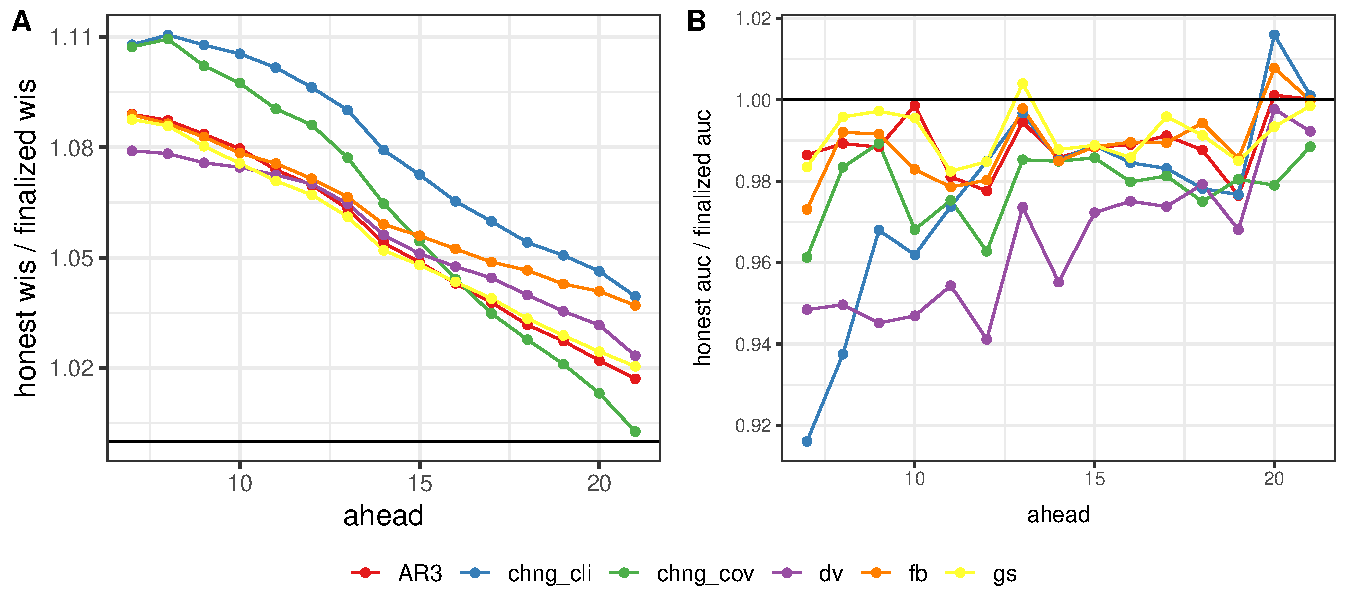
\includegraphics[width=\linewidth]{fig/figure6.pdf}
     \caption{How misleading is a retrospective analysis that uses the
       finalized version of the data rather than the version that was
       in fact available at the time the forecast was made?  Plots
       show the ratio in performance (using mean WIS fore the
       forecasting task and AUC for the hotspot prediction
       task). \label{fig:finalized-vs-honest} Cheating vs. honest plots.} 
\end{figure}

\subsection{Additional sensitivity analyses}

In addition to whether one properly accounts for signal latency, there
are several other choices in evaluating forecasters that can also have
a non-trivial impact on results.

For example, in Figure
\ref{fig:topline-overall-results}, we show the ratio
of means.  Other choices of aggregation and scaling are also
possible.  For example, taking the mean of ratios of errors is
possible and would give more importance to locations where
errors are small (either because the location-time pairs had low case
rates or because the forecasting task was itself easier).  By
contrast, the ratio of the mean of errors may be dominated by
location-time pairs where the error is large.
Figure \ref{fig:
  scale-aggregate-order} of the Supplementary Information shows...
\begin{itemize}
\item Note the y-axis: barely an improvement over baseline, and this goes away for AR after 11 days ahead, and for all other models around 13-14 days ahead.
\item Using trimmed means here because otherwise the results are extremely unstable (as the denominators can be small, when WIS of baseline is small).
\item Similar message to before (non-adjusted), but \dv~and \chngcov~the best, \fb~and \gs~still good, but now \chngcli~seems to do much better!  
\item What's our interpretation here?  That somehow \chngcli~just
  does particularly bad in tasks where the baseline is also bad?
  \item We might include a histogram of WIS with a log-transformed
    x-axis to suggest that the geometric mean may be reasonable here.
\end{itemize}
Using instead the geometric mean makes the order of aggregation and
scaling immaterial since the ratio of geometric means is the same as
the geometric mean of ratios.  Figure \ref{fig:geometric-mean} of the
Supplementary Information shows how Figure
\ref{fig:topline-overall-results} panel A would change if
one replaces the arithmetic mean by the geometric mean.

In Supplementary Information \ref{sec:2021}, we investigate the effect of lengthening
the time window to include 2021.
\begin{itemize}
\item For forecasting: results get better, whether we look at
  non-adjusted (first plot) or adjusted scores (second plot).  Other
  than that, interpretation is qualitatively similar, except fb now
  seems to be worse than gs.  And \chngcli~is strong, even in the
  non-adjusted view.
  \item For hotspots: Alden will write something explaining why we
    don't do hotspot detection in 2021.
\end{itemize}

In Supplementary Information Section \ref{sec:gs-locations}, we look at various approaches to
accounting for the fact that the \gs~indicator is only available
for XX HRRs.

\begin{itemize}
  \item For forecasting task: clearly gs is not missing at random, and when it's present, it tends to be predictive.  Hence high values have a low false positivity rate.  Most visible in the adjusted view below, where gs triumphs.  Also \chngcli~gets a lot worse.

\item For hotspots: All methods look better, suggesting that the “GS locations” are easier for hotspot prediction. E.g. at 7-days ahead, the AUCs computed based on all locations range from 0.61-0.66; restricted to GS locations, the AUCs range from about 0.65-0.69. (These are all eyeballed, should get actual numbers if we want to say something like this in paper.)
\item gs\_subset appears to be particularly helped by this subsetting
  (which makes sense since on those other locations it was 0-imputed)
  \item Daniel will also try gs\_impute as in forecasting
\end{itemize}

% Figure \ref{fig:forecast-median-relative-wis-faceted} splits the topline
% median relative WIS results over four time periods:  June and July, which
% corresponds to the small, initial surge experienced in the US;
% August and September, when incident cases nationally were somewhat stable;
% October, when a second surge was witnessed; and November and December,
% which saw the largest surges to date.  In essentially all the time periods,
% the indicator-assisted models perform in aggregate as well or better than
% the baseline QAR3 model.  The results in October do not show much
% differentiation between the baseline QAR3 and the indicator-assisted models.
% However, we note that during that time period, even the baseline QAR3
% model is doing very well in terms of relative WIS (especially compared to
% other time periods), so perhaps there is not much ``room for improvement'',
% so to speak.

% \begin{figure*}[tb!]
%      \centering
%      \begin{subfigure}[b]{0.49\textwidth}
%          \centering
%          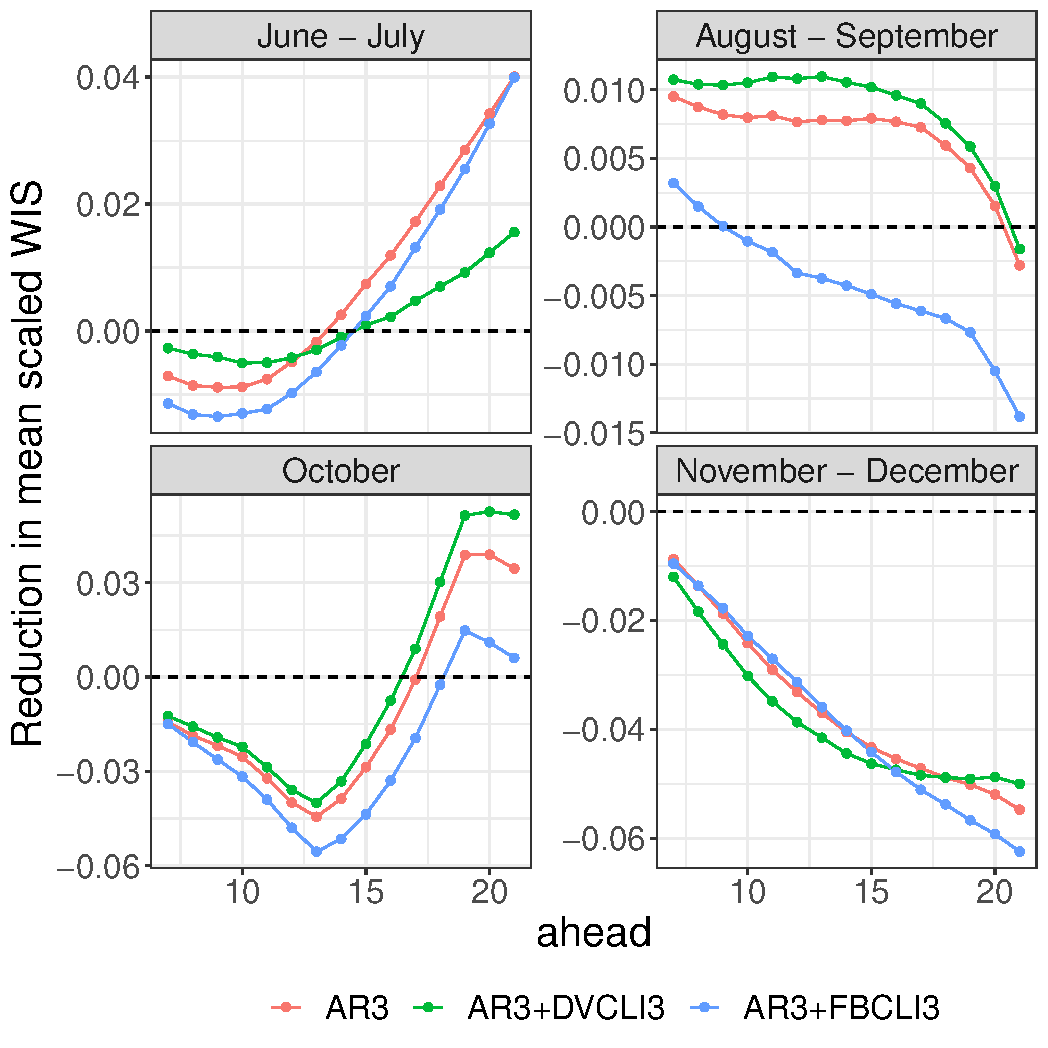
\includegraphics[width=\textwidth]{fig/reduction_mean_scaled_wis_facet_honest.pdf}
%          \caption{Forecasting task: mean WIS relative to mean WIS of baseline}
%          \label{fig:forecast-reduction-mean-scaled-wis-facet}
%      \end{subfigure}
%      \hfill
%      \begin{subfigure}[b]{0.49\textwidth}
%          \centering
%          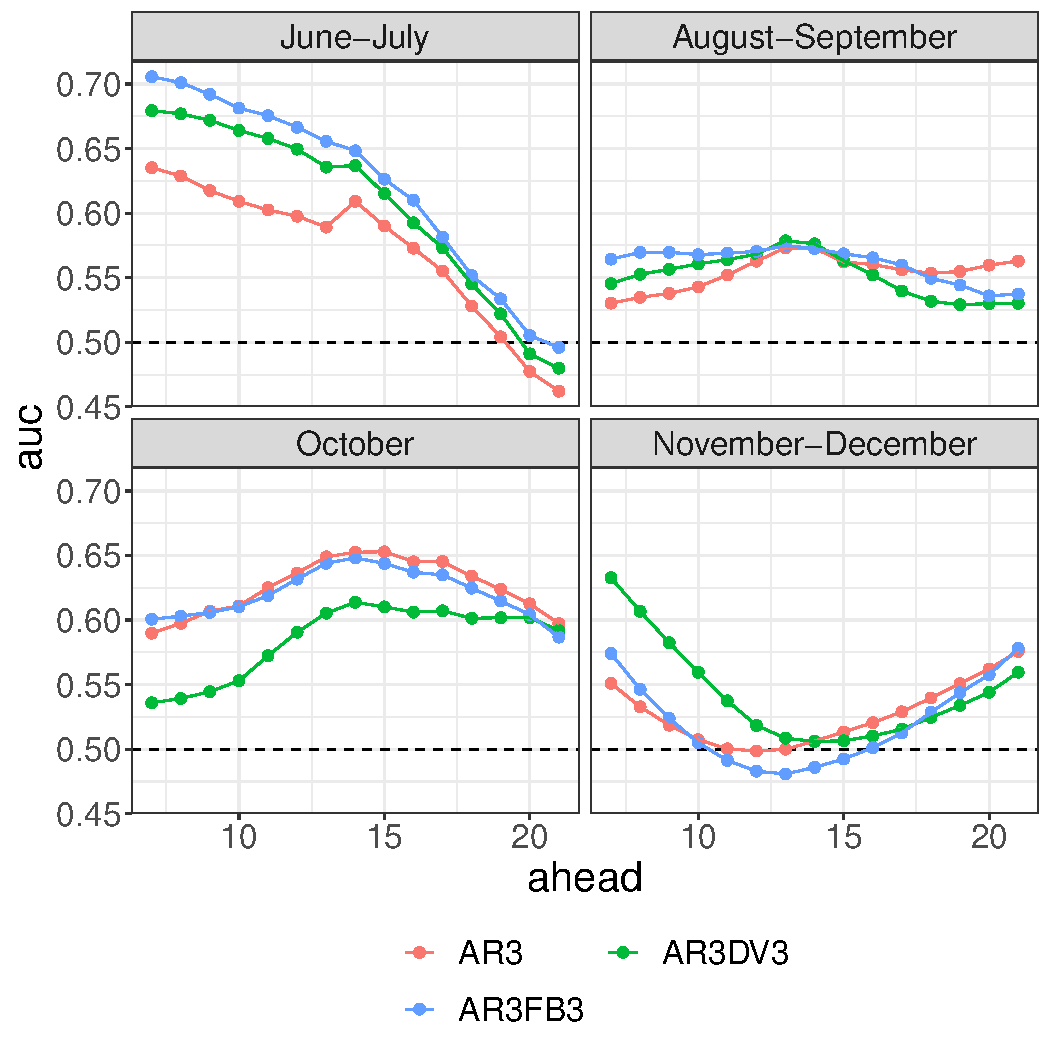
\includegraphics[width=\textwidth]{fig/auc_by_forecast_period.pdf}
%          \caption{Hotspot prediction task: AUC}
%          \label{fig:hotspot-auc-faceted}
%      \end{subfigure}
%      \label{fig:topline-faceted-results}
%      \caption{Topline results from June - December 2020, split into
%      four representative time periods.}
% \end{figure*}


\paragraph{\attn{Additional results section material, some for Discussion}}


\begin{figure}
    \centering
    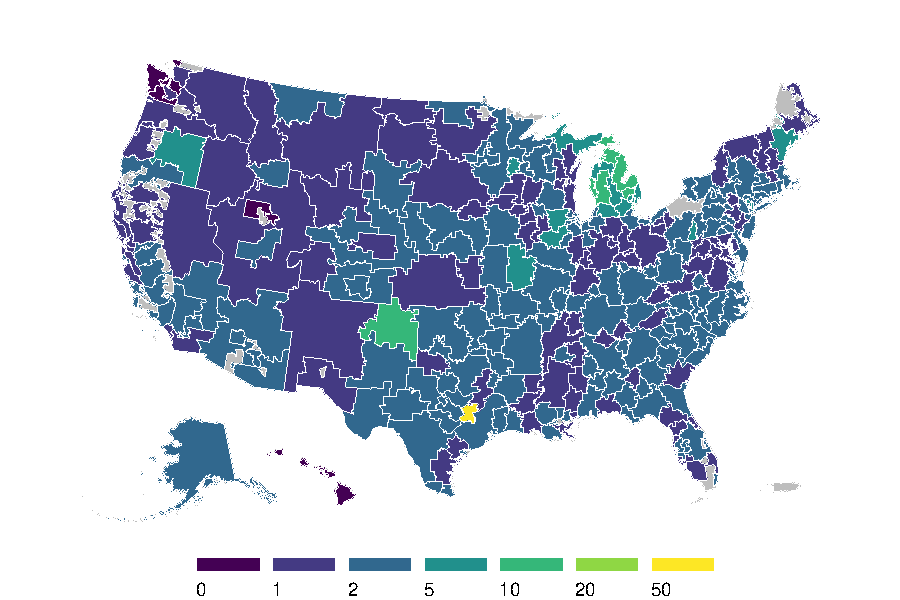
\includegraphics[width=.95\linewidth]{fig/fake-map.pdf}
    \caption{Weighted interval score for forecasts made on April 1, 2021. Scores
      are averaged over horizons from 1 to 14 days ahead and are relative to
      population size.} 
    \label{fig:fake-map}
\end{figure}

\begin{enumerate}
%\item How does this vary over time? Table showing 7-day ahead and 14-day ahead
%  (just picking out two of the d=5,...,20). Include a national curve.
\item Spatial map of errors across HRRs for both tasks. See
  \autoref{fig:fake-map} for an example. 
\item Unlikely we can find it, but we should try anyway. Possibly put in the
  intro or discussion instead. Find an example of a forecast altered by the
  presence of an indicator.  Plot the two trajectories.
\item Examine a specific HRR over time. What does it mean to predict certain
  hotspots? How can we understand what is happening?
 \item What can we say about statistical significance? NRI, paired t-test?
 \item Figures showing hotspots make sense
 \item Horizontal line at 0.5 on AUC curve, discribe that this is random
   guessing. 
\end{enumerate}


\section{Discussion}

We have assessed the performance of [NUMBER] indicators in terms of their
usefulness for performing two forecasting tasks: probabilistic
forecasting of case
rates and hotspot prediction at the HRR-level, 1--[NUMBER] days in advance.
In measuring the practical usefulness of an indicator to forecasting,
we distinguish between honest versus aspirational assessments.  Data
latency is an important factor when considering the usefulness of an
indicator.  Retrospective evaluations that ignore these messy data
issues fail to provide the full picture.  While one can hope that reporting
systems will operate faster and more consistently in ``the next
pandemic,'' some reasons for this latency appear unavoidable.  The
chaos and strain inherent to pandemic times make indicators that can
be reported and collected with quickly with minimal effort or manual
involvement desirable.

We conclude by observing that the
approach we have taken in this paper is somewhat opposite to that of much of the COVID-19
forecasting literature.  We have chosen to consider only very simple forecasting models while devoting most of our effort to accounting for as much of the complexity of
the data and evaluation as possible.  By contrast, many papers focus
on very complicated forecasting approaches but then evaluate them
under unrealistic, retrospective conditions.


\begin{enumerate}

\item Discussion should contain more detailed lit review ("context"), rather
  than in the intro, per the instructions. 

\item Use of syndromic surveillance for other diseases?

\item Cite any papers that use our signals in forecasting.
\end{enumerate}

\paragraph{\attn{Other potential discussion topics}}



\begin{itemize}

\item When was this data actually available? (As of issue. The argument is: sure
  we didn't have it, but it would have helped. We should have this next time.)
\item Side issues, are there places / times where one signal is especially good?
  Especially bad?
\item What do we do about holidays? How do we understand the performance when
  the data is trash? If the data is trash, all the more reason to have other
  data that is perhaps less susceptible to these criticisms.
\item Other signals we might want? Mobility? Discuss how SEIR models need
  contact matrices, relationship with ``in community'' signals.
  
\end{itemize}

\showmatmethods{} % Display the Materials and Methods section

\acknow{Please include your acknowledgments here, set in a single paragraph. Please do not include any acknowledgments in the Supporting Information, or anywhere else in the manuscript.}

\showacknow{} % Display the acknowledgments section

% Bibliography
\bibliography{../../common/covidcast.bib}

\end{document}
